%
%Не забыть:
%--------------------------------------
%Вставить колонтитулы, поменять название на титульнике



%--------------------------------------

\documentclass[a4paper, 12pt]{article} 

%--------------------------------------
%Russian-specific packages
%--------------------------------------
%\usepackage[warn]{mathtext}
\usepackage[T2A]{fontenc}
\usepackage[utf8]{inputenc}
\usepackage[english,russian]{babel}
\usepackage[intlimits]{amsmath}
\usepackage{esint}
%--------------------------------------
%Hyphenation rules
%--------------------------------------
\usepackage{hyphenat}
\hyphenation{ма-те-ма-ти-ка вос-ста-нав-ли-вать}
%--------------------------------------
%Packages
%--------------------------------------
\usepackage{amsmath}
\usepackage{amssymb}
\usepackage{amsfonts}
\usepackage{amsthm}
\usepackage{latexsym}
\usepackage{mathtools}
\usepackage{etoolbox}%Булевые операторы
\usepackage{extsizes}%Выставление произвольного шрифта в \documentclass
\usepackage{geometry}%Разметка листа
\usepackage{indentfirst}
\usepackage{wrapfig}%Создание обтекаемых текстом объектов
\usepackage{fancyhdr}%Создание колонтитулов
\usepackage{setspace}%Настройка интерлиньяжа
\usepackage{lastpage}%Вывод номера последней страницы в документе, \lastpage
\usepackage{soul}%Изменение параметров начертания
\usepackage{hyperref}%Две строчки с настройкой гиперссылок внутри получаеммого
\usepackage[usenames,dvipsnames,svgnames,table,rgb]{xcolor}% pdf-документа
\usepackage{multicol}%Позволяет писать текст в несколько колонок
\usepackage{cite}%Работа с библиографией
\usepackage{subfigure}% Человеческая вставка нескольких картинок
\usepackage{tikz}%Рисование рисунков
\usepackage{float}% Возможность ставить H в положениях картинки
\usepackage{braket}% Бра-кет вектора
% Для картинок Моти
\usepackage{misccorr}
\usepackage{lscape}
\usepackage{cmap}



\usepackage{graphicx,xcolor}
\graphicspath{{Pictures/}}
\DeclareGraphicsExtensions{.pdf,.png,.jpg}

%----------------------------------------
%Список окружений
%----------------------------------------
\newenvironment {theor}[2]
{\smallskip \par \textbf{#1.} \textit{#2}  \par $\blacktriangleleft$}
{\flushright{$\blacktriangleright$} \medskip \par} %лемма/теорема с доказательством
\newenvironment {proofn}
{\par $\blacktriangleleft$}
{$\blacktriangleright$ \par} %доказательство
%----------------------------------------
%Список команд
%----------------------------------------
\newcommand{\grad}
{\mathop{\mathrm{grad}}\nolimits\,} %градиент

\newcommand{\diver}
{\mathop{\mathrm{div}}\nolimits\,} %дивергенция

\newcommand{\rot}
{\ensuremath{\mathrm{rot}}\,}

\newcommand{\Def}[1]
{\underline{\textbf{#1}}} %определение

\newcommand{\RN}[1]
{\MakeUppercase{\romannumeral #1}} %римские цифры

\newcommand {\theornp}[2]
{\textbf{#1.} \textit{ #2} \par} %Написание леммы/теоремы без доказательства

\newcommand{\qrq}
{\ensuremath{\quad \Rightarrow \quad}} %Человеческий знак следствия

\newcommand{\qlrq}
{\ensuremath{\quad \Leftrightarrow \quad}} %Человеческий знак равносильности

\renewcommand{\phi}{\varphi} %Нормальный знак фи

\newcommand{\me}
{\ensuremath{\mathbb{E}}}

\newcommand{\md}
{\ensuremath{\mathbb{D}}}

\newcommand{\med}[1]
{\ensuremath{\langle#1\rangle}}



%\renewcommand{\vec}{\overline}




%----------------------------------------
%Разметка листа
%----------------------------------------
\geometry{top = 3cm}
\geometry{bottom = 2cm}
\geometry{left = 1.5cm}
\geometry{right = 1.5cm}
%----------------------------------------
%Колонтитулы
%----------------------------------------
\pagestyle{fancy}%Создание колонтитулов
\fancyhead{}
%\fancyfoot{}
%----------------------------------------
%Интерлиньяж (расстояния между строчками)
%----------------------------------------
%\onehalfspacing -- интерлиньяж 1.5
%\doublespacing -- интерлиньяж 2
%----------------------------------------
%Настройка гиперссылок
%----------------------------------------
\hypersetup{				% Гиперссылки
	unicode=true,           % русские буквы в раздела PDF
	pdftitle={Заголовок},   % Заголовок
	pdfauthor={Автор},      % Автор
	pdfsubject={Тема},      % Тема
	pdfcreator={Создатель}, % Создатель
	pdfproducer={Производитель}, % Производитель
	pdfkeywords={keyword1} {key2} {key3}, % Ключевые слова
	colorlinks=true,       	% false: ссылки в рамках; true: цветные ссылки
	linkcolor=blue,          % внутренние ссылки
	citecolor=blue,        % на библиографию
	filecolor=magenta,      % на файлы
	urlcolor=cyan           % на URL
}
%----------------------------------------
%Работа с библиографией (как бич)
%----------------------------------------
\renewcommand{\refname}{Список литературы}%Изменение названия списка литературы для article
%\renewcommand{\bibname}{Список литературы}%Изменение названия списка литературы для book и report
%----------------------------------------
\begin{document}
	\begin{titlepage}
		\begin{center}
			$$$$
			$$$$
			$$$$
			$$$$
			{\Large{НАЦИОНАЛЬНЫЙ ИССЛЕДОВАТЕЛЬСКИЙ УНИВЕРСИТЕТ}}\\
			\vspace{0.1cm}
			{\Large{ВЫСШАЯ ШКОЛА ЭКОНОМИКИ}}\\
			\vspace{0.25cm}
			{\large{Факультет физики}}\\
			\vspace{5.5cm}
			{\Huge\textbf{{Домашние работы по первой части курса}}}\\%Общее название
			\vspace{2cm}
			{Работу выполнил студент 3 курса}\\
			{Захаров Сергей Дмитриевич}\\
			\vfill
			
\includegraphics[width = 0.2\textwidth]{HSElogo}\\
			\vfill
			Москва\\
			2021
		\end{center}
	\end{titlepage}
	
\tableofcontents


\newpage

\section{Неделя 1}

\subsection{\textit{Для ОЦК и ГЦК решеток найти вектора примитивных трансляций и ячейку Вигнера-Зейтца. Найти обратные решетки.}}

\subsubsection{Вектора примитивных трансляций ОЦК}

\begin{align}
	v_1 &= \begin{pmatrix}
		0 \\ 0 \\ a
	\end{pmatrix}
	+ \frac{1}{2\sqrt{3}}\begin{pmatrix}
		a \\ a \\ a
	\end{pmatrix} = \frac{a}{2\sqrt{3}} \begin{pmatrix}
	1 \\ 1 \\ 2\sqrt{3} + 1
\end{pmatrix}\\
	v_2 &= \frac{a}{2\sqrt{3}} \begin{pmatrix}
	1 \\ 2\sqrt{3} + 1 \\ 1
\end{pmatrix}\\
	v_3 &= \frac{a}{2\sqrt{3}} \begin{pmatrix}
		2\sqrt{3} + 1 \\ 1 \\ 1
	\end{pmatrix}
\end{align}

\subsubsection{Вектора примитивных трансляций ГЦК}

\begin{align}
	v_1 &= \frac{a}{\sqrt{2}}\begin{pmatrix}
		1 \\ 1 \\ 0
	\end{pmatrix}\\
	v_2 &= \frac{a}{\sqrt{2}} \begin{pmatrix}
		1 \\ 0 \\ 1
	\end{pmatrix}\\
	v_3 &= \frac{a}{\sqrt{2}} \begin{pmatrix}
		0 \\ 1 \\ 1
	\end{pmatrix}
\end{align}

\subsubsection{Ячейка Вигнера-Зейтца ОЦК}

Для произвольного узла (взял центральный) строим отрезки до ближайших узлов. Через их середины, перпендикулярно им, проводим плоскости. Пересечение всех этих плоскостей даст искомую ячейку. Опустив расчеты точек приведем только красивую картинку:

\begin{figure}[H]
	\centering
	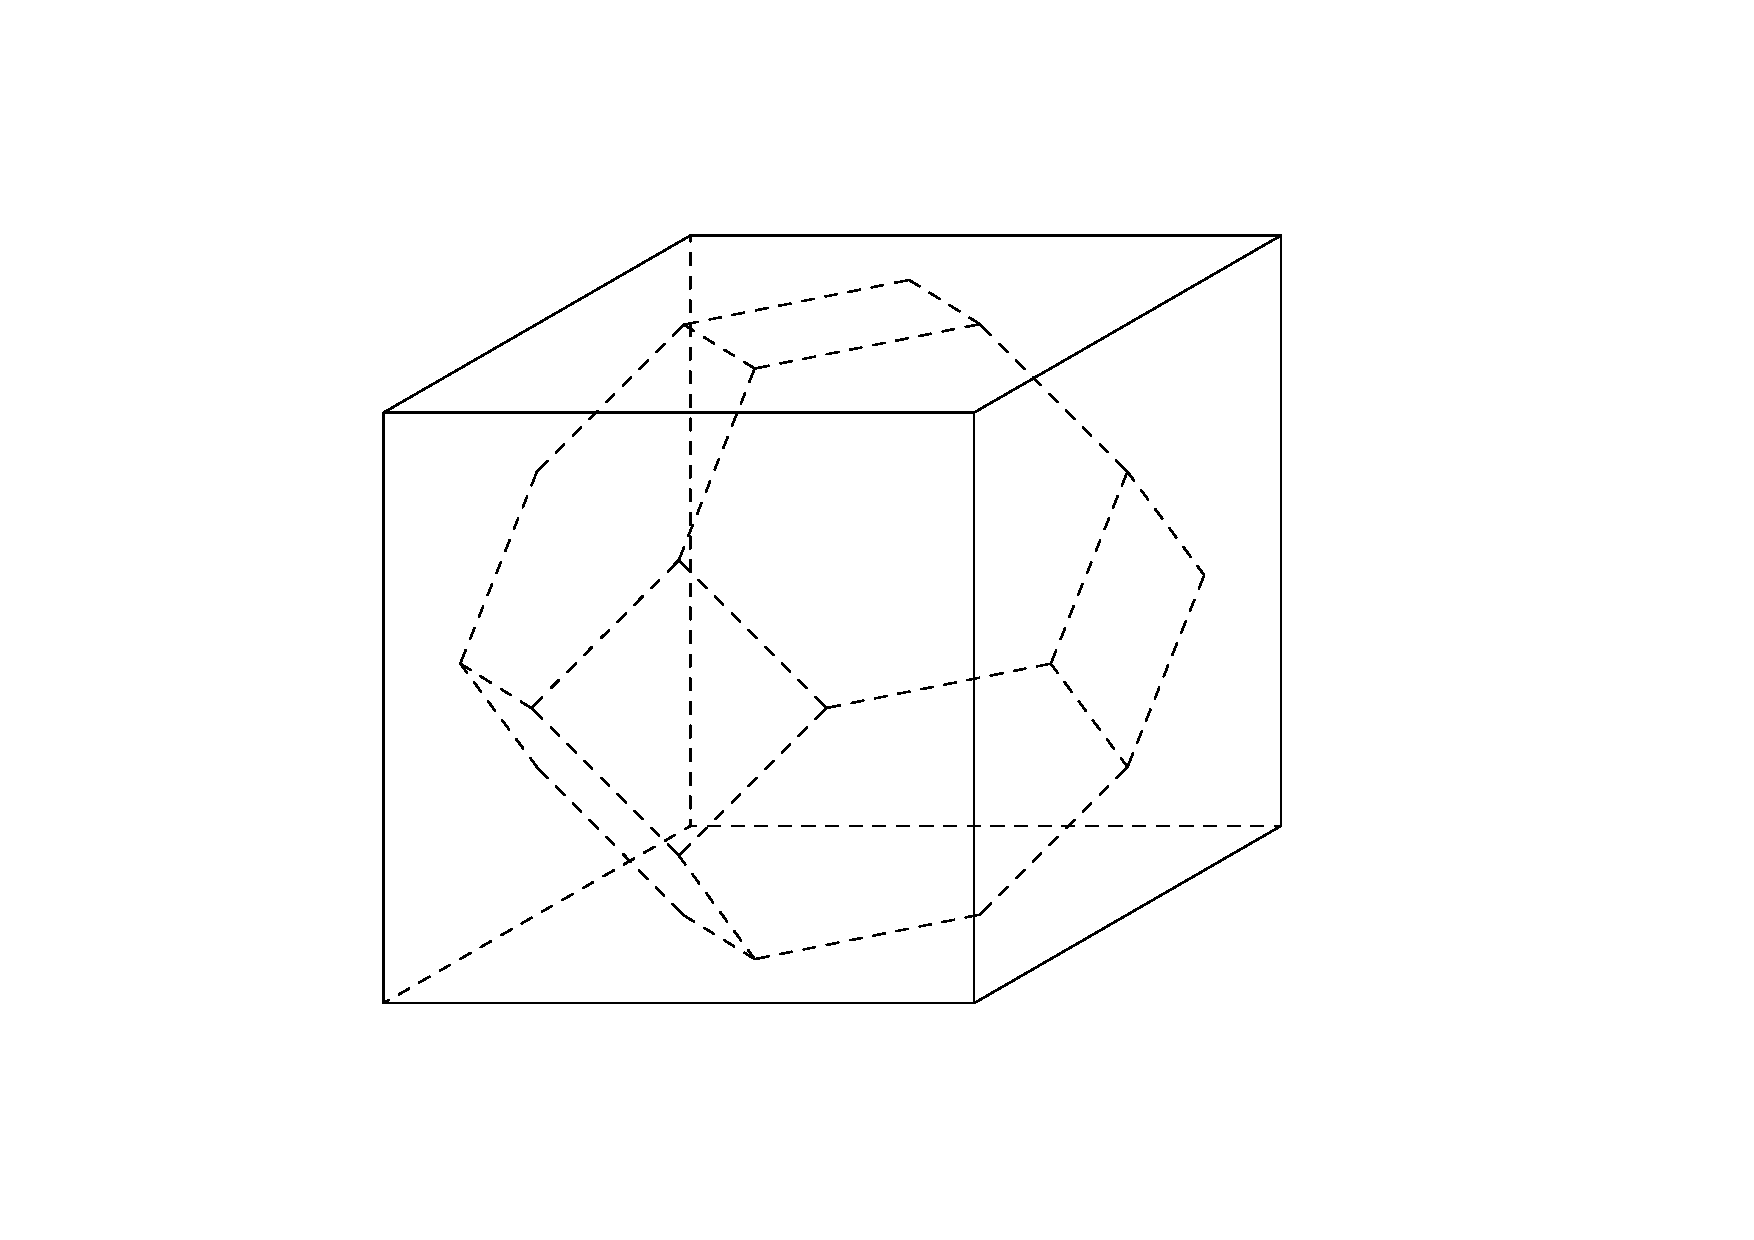
\includegraphics[width=0.8\linewidth]{1_OCK}
	\caption{Ячейка Вигнера-Зейтца для ОЦК решетки}
\end{figure}

\subsubsection{Ячейка Вигнера-Зейтца ГЦК}

Все то же самое, но для ГЦК.

\begin{figure}[H]
	\centering
	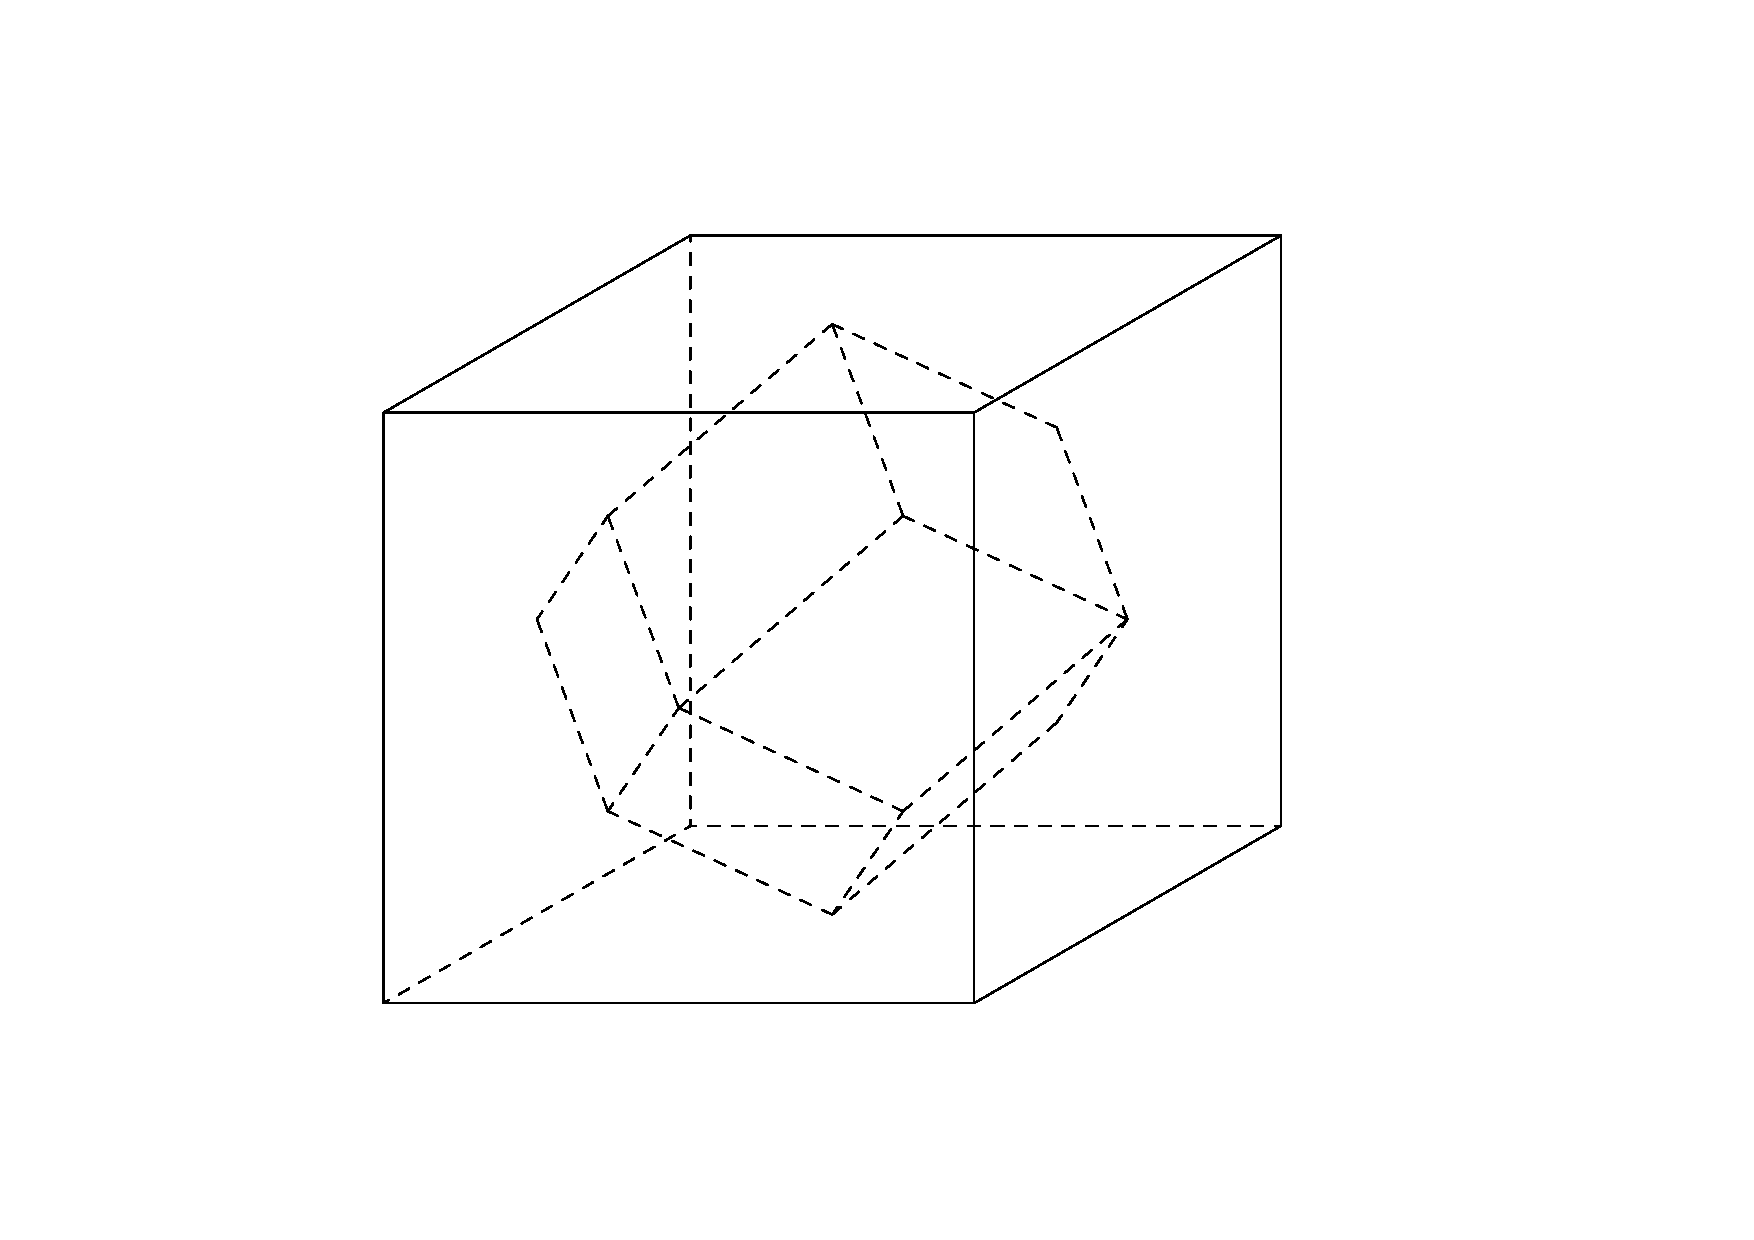
\includegraphics[width=0.8\linewidth]{1_GCK}
	\caption{Ячейка Вигнера-Зейтца для ГЦК решетки}
\end{figure}

\subsubsection{Обратная решетка ОЦК}

Возьмем в качестве базиса, например:

\begin{equation}
	a_1 = 
	\begin{pmatrix}
	1 \\ 0 \\ 0
	\end{pmatrix}, \quad
	a_2 = 
	\begin{pmatrix}
		0 \\ 1 \\ 0
	\end{pmatrix}, \quad
	a_3 = 
	\begin{pmatrix}
		1/2 \\ 1/2 \\ 1/2
	\end{pmatrix}	
\end{equation}

Для обратной решетки сперва посчитаем:

\begin{equation}
	a_1 \cdot [a_2 \times a_3] = 
	\begin{vmatrix}
		1 & 0 & 0 \\
		0 & 1 & 0 \\
		\dfrac{1}{2} & \dfrac{1}{2} & \dfrac{1}{2} 
	\end{vmatrix} = \frac{1}{2}
\end{equation}

Тогда для векторов:

\begin{align}
	b_1 &= 2\pi \frac{[a_2 \times a_3]}{1/2} = 2\pi \cdot
	\begin{pmatrix}
		1 \\ 0 \\ -1
	\end{pmatrix}\\
	b_2 &= 2\pi \frac{[a_3 \times a_1]}{1/2} = 2\pi \cdot
	\begin{pmatrix}
		0 \\ 1 \\ -1
	\end{pmatrix}\\
	b_3 &= 2\pi \frac{[a_1 \times a_2]}{1/2} = 2\pi \cdot
	\begin{pmatrix}
		0 \\ 0 \\ 2
	\end{pmatrix}
\end{align}

\subsubsection{Обратная решетка ГЦК}

\begin{equation}
	a_1 = 
	\begin{pmatrix}
		1/2 \\ 1/2 \\ 0
	\end{pmatrix}, \quad
	a_2 = 
	\begin{pmatrix}
		0 \\ 1/2 \\ 1/2
	\end{pmatrix}, \quad
	a_3 = 
	\begin{pmatrix}
		1/2 \\ 0 \\ 1/2
	\end{pmatrix}	
\end{equation}

Для обратной решетки посчитаем:

\begin{equation}
	a_1 \cdot [a_2 \times a_3] =  \frac{1}{4}
\end{equation}

\begin{align}
	b_1 &= 2\pi \frac{[a_2 \times a_3]}{1/4} = 2\pi \cdot
	\begin{pmatrix}
		1 \\ 1 \\ -1
	\end{pmatrix}\\
	b_2 &= 2\pi \frac{[a_3 \times a_1]}{1/4} = 2\pi \cdot
	\begin{pmatrix}
		-1 \\ 1 \\ 1
	\end{pmatrix}\\
	b_3 &= 2\pi \frac{[a_1 \times a_2]}{1/4} = 2\pi \cdot
	\begin{pmatrix}
		1 \\ -1 \\ 1
	\end{pmatrix}
\end{align}

\newpage

\section{Неделя 2}

\subsection{\textit{Показать, что амплитуда колебаний тела на пружинке (горизонтальное движение) в пределе $\omega \gg \omega_0 = \sqrt{k/m}$ не зависит от частоты и совпадает с амплитудой свободного тела без пружинки}}

Запишем второй закон Ньютона для осциллятора на пружинке (пружина = наличие внешней силы):

\begin{equation}
	ma = -kx + F_0\cos(\omega t)
\end{equation}

Введем следующие обозначения:

\begin{equation}
	\omega_0^2 = \frac{k}{m}, \quad \Phi_0 = \frac{F_0}{m}
\end{equation}

Заменим ускорение на законную вторую производную координаты по времени, получим дифур:

\begin{equation}
	\ddot{x} + \omega^2 x = \Phi_0 \cos(\omega t)
\end{equation}

Решение будем искать как сумму общего решения однородного уравнения и частного решения неоднородное. Общее решение мы уже знаем, оно имеет вид:

\begin{equation}
	x(t) = A \sin(\omega_0 t + \phi_0)
\end{equation}

Чтобы найти частное решение подставим в уравнение решение вида $x(t) = B \cos(\omega t)$ и найдем константу:

\begin{equation}
	B = \frac{\Phi_0}{\omega_0^2 - \omega^2}
\end{equation}

В таком случае окончательное решение имеет вид:

\begin{equation}
	x(t) = A\sin(\omega_0 + \phi_0) + \frac{\Phi_0}{\omega_0^2 - \omega^2} \cos(\omega t)
\end{equation}

В интересующем нас случае мы можем вторым членом пренебречь: частота колебаний косинуса будет очень высокой (по сравнению с частотой изменения синуса). Поэтому мы можем формально усреднить по небольшому периоду колебаний косинуса, не трогая при этом усреднении синус, и получить, что $x(t) = A\sin(\omega + \phi_0)$ не зависит от $\omega$, а амплитуда совпадает с амплитудой без пружинки.

\newpage

\section{Неделя 3}

\subsection{\textit{Посчитать $\langle \Delta x^2 \rangle$ для гармонического осциллятора}}

Запишем равенство энергий:

\begin{equation}
	\frac{k \langle \Delta x^2 \rangle}{2} = \frac{k_B T}{2} \qrq \left[k = m \omega^2\right] \qrq \langle \Delta x^2 \rangle = \frac{k_B T}{m \omega^2} \approx 4.14 \cdot 10^{-21} \text{ м}
\end{equation}

\subsection{\textit{Определить структурный фактор ГЦК решетки}}

Базис выберем следующий:

\begin{equation}
\begin{pmatrix}
	0 & 0 & 0
\end{pmatrix}, \quad
\begin{pmatrix}
	1/2 & 1/2  & 0
\end{pmatrix}, \quad
\begin{pmatrix}
	0 & 1/2 & 1/2
\end{pmatrix}, \quad
\begin{pmatrix}
	1/2 & 0 & 1/2 
\end{pmatrix}
\end{equation}

\begin{align*}
	S(h, k, l) = \sum\limits_i f_i e^{-2 i \pi (x_i h + y_i k + z_i l)} = f\left(1 + e^{-2 i \pi (h/2 + k/2)} + e^{-2i\pi(h/2 + l/2)} + e^{-2i\pi(k/2 + l/2)}\right) = \\
	= f(1 + e^{-i\pi(h + k)} + e^{-i\pi} + e^{-i\pi(k + l)} + e^{-i\pi(h + l)})
\end{align*}

Положим, что все индексы имеют одинаковую четность. Тогда попарные суммы, стоящие в экспонентах, тоже все четные, из-за чего экспоненты оказываются равными единице, а $S = 4f$.

Если же теперь предположить, что одинаковую четность имеют только два из трех (не важно, каких) индекса, то только одна экспонента окажется равно 1, а две другие --- $-1$. В таком случае $S = 0$.

\subsection{\textit{Определить структурный фактор ОЦК решетки}} 

Базис выберем следующий:

\begin{equation}
\begin{pmatrix}
	0 & 0 & 0
\end{pmatrix}, \quad
\begin{pmatrix}
	1/2 & 1/2 & 1/2
\end{pmatrix}
\end{equation}


Запишем структурный фактор:

\begin{equation}
	S (h, k, l) = \sum\limits_i f_i e^{-2i\pi (x_i h + y_i k + z_i l)} = f(1 + e^{-i\pi (h + k + l)})
\end{equation}

Вновь, как в прошлой задаче, возможно два случая. Сперва предположим, что сумма трех индексов есть число четное, то экспонента даст 1, и, следовательно, $S = 2f$.

В противном случае экспонента даст $-1$, и $S = 0$.

\newpage

\section{Неделя 4}

\subsection{\textit{Рассчитать вклад оптической ветви колебаний в теплоемкость~$c_V$}}

Положим $\omega = \omega_0 + \omega_1 \cos(k a)$, при условии $\omega_0 \gg \omega_1$, а $\omega_0 \gg \theta$.

Тогда $E = 3 \sum\limits_k E(k) N(k)$, $\varepsilon =  \hbar \omega_k (n(\varepsilon) + 1/2)$. $\hbar$ в дальнейшем будем опускать, а $n(\varepsilon)$ соответствует $f_B(\varepsilon)$.

Если $\omega \approx \omega_0$, то:

\begin{equation}
	f_B = \frac{1}{e^{\omega/T} - 1} \approx \frac{1}{e^{\omega_0/T} - 1} \quad \text{--- заменим на константу}
\end{equation}

Тогда:

\begin{equation}
	E = 3 N(V) \omega_0 \left(\frac{1}{e^{\omega_0/T} - 1} + \frac{1}{2}\right) \qrq c_V = \left(\frac{\partial E}{\partial T}\right)_V = \frac{3 N \omega_0^2}{T^2} \cdot \frac{e^{\omega_0 / T}}{(e^{\omega_0 / T} - 1)^2}
\end{equation}

Рассмотрим различные случаи.

\subsubsection{$T \ll \theta \ll \omega_0$:}

\begin{equation}
	c_V^{\text{акк}} \propto \left(\frac{T}{\theta}\right)^3, \quad c_V^{\text{опт}} \propto \left(\frac{\omega_0}{T}\right)^2 e^{-2 \omega_0 / T} \qrq \frac{c_V^{\text{опт}}}{c_V^{\text{акк}}} \propto e^{-2\omega_0 / T}
\end{equation}

\subsubsection{$T \gg \theta, T \sim \omega_0$:}

\begin{equation}
	c_V^{\text{акк}} \approx 3N, \quad c_V^{\text{опт}} \approx 3N \qrq \frac{c_V^{\text{опт}}}{c_V^{\text{акк}}} \sim 1
\end{equation}

\subsubsection{$T \gg \theta, T \sim \omega_0$:}

\begin{equation}
	c_V^{\text{акк}} = 3 N, \quad c_V^{\text{опт}} = 3N \frac{\omega_0^2}{T^2} \qrq \frac{c_V^{\text{опт}}}{c_V^{\text{акк}}} \sim \left(\frac{\omega_0}{T}\right)^2
\end{equation}

\subsection{\textit{Выразить $\mu_B$ через фундаментальные константы, рассмотрев магнитный момент, возникающий за счет орбитального движения электрона}}

Если рассмотреть электрон как некоторый заряд, который движется по круговой орбите, то его магнитный момент:

\begin{equation}
	\mu = \frac{I S}{c} = \frac{e v}{2 \pi R} \cdot \frac{\pi R^ 2}{c} = \frac{e m v R}{2 m c} = \frac{e M}{2 m c}
	\label{eq:4_mu}
\end{equation}

Механический момент квантуется как $M = l \hbar$. Тогда из \ref{eq:4_mu} получим:

\begin{equation}
	\mu = \frac{e \hbar l}{2 m_e c} = \mu_B l \qrq \mu_B = \frac{e \hbar}{2 m_e c}
\end{equation}

\subsection{\textit{Найти теплоемкость системы осцилляторов с частотой $\omega_0$ при температуре $T$}}

Для удобства (чтобы как в прошлой задаче не таскать $T$ в знаменателе) перебросим $T$ в $\beta = 1/T$.

\subsubsection{Одномерье}

Путь у нас есть $N$ невозмущенных осцилляторов, тогда:

\begin{equation}
	Z_1 = \sum\limits_{n=0}^\infty e^{-\hbar \beta \omega_0 (n + 1/2)} = e^{-\hbar \beta \omega_0 / 2} \frac{1}{1 - e^{-\hbar \beta \omega_0}} = \frac{1}{2 \sinh(\hbar \beta \omega_0  /2)}
\end{equation}

Тогда для $Z$ можно записать:

\begin{equation}
	Z = \frac{1}{2^N \sinh^N(\hbar \beta \omega_0 / 2)} \qrq  F  = - T \ln Z = - T N \ln \left(\frac{1}{2\sinh(\hbar \beta \omega_0 / 2)}\right)
\end{equation}

Тогда при $T\rightarrow 0$ для $c$ можно записать:

\begin{equation}
	c = - T \frac{\partial^2 F}{\partial T^2} = \frac{N \hbar^2 \omega^2}{\sinh^2[\hbar \omega_0 / (2 T)]}
\end{equation}

\subsubsection{Трехмерье}

Действуем аналогично. Для $Z_1$:

\begin{equation}
	Z_1 = e^{-3\hbar\beta \omega_0 / 2} \sum\limits_{n, k, l} e^{-(n + k + l) \hbar \beta \omega_0} = \frac{1}{8 \sinh^3(\hbar\beta\omega_0/2)}
\end{equation}

Отсюда в целом сразу следует осознание, что трехмерная $c_3$ равна трем одномерным $c_1$:

\begin{equation}
	c_3 = 3 c_1
\end{equation} 

\newpage

\section{Неделя 7}

\subsection{\textit{Найти $M = M_1 + M_2 = f(T)$}}

\begin{equation}
	\begin{cases*}
		M_1 = \dfrac{c}{T}(H + \lambda M_2)\\
		M_2 = \dfrac{c}{T}(H + \lambda M_1)
	\end{cases*}
	\qrq M = (M_1 + M_2) = \frac{2 c H}{T} \frac{1}{1 - \dfrac{c\lambda}{T}} \qrq \chi = \frac{M}{H} = \frac{2c}{T - c\lambda}
\end{equation}

\subsection{\textit{Показать, что $\hat{S}_1 \hat{S}_2 = S_1^z S_2^z + (S_1^+S_2^- + S_1^-S_2^+)/2$}}

Запишем для $\hat{S}_1 \hat{S}_2$:

\begin{equation}
	\hat{S}_1 \hat{S}_2 = S_1^x S_2^x + S_1^y S_2^y + S_1^z S_2^z
	\label{eq:7_ss}
\end{equation}

Распишем $S^+, S^-$:

\begin{align}
	S^+ = S^x + i S^y\\
	S^- = S^x - i S^y
\end{align}

Распишем $S_1^+S_2^-$, $S_1^-S_2^+$:

\begin{align}
	S_1^+S_2^- = (S_1^x + iS_1^y)(S_2^x - iS_2^y) = S_1^x S_2^x + S_1^yS_2^y - i S_1^x S_2^y + i S_1^y S_2^x\\
	S_1^-S_2^+ = (S_1^x - iS_1^y)(S_2^x + iS_2^y) = S_1^x S_2^x + S_1^yS_2^y - i S_1^y S_2^x + i S_1^x S_2^y
\end{align}

Тогда из \ref{eq:7_ss} получаем:

\begin{equation}
	\hat{S}_1 \hat{S}_2 = S_1^x S_2^x + S_1^y S_2^y + S_1^z S_2^z = S_1^z + S_2^z  \frac{1}{2} (S_1^+S_2^- + S_1^-S_2^+)
\end{equation}


\newpage

\subsection{\textit{Изучается рассеянный под углом 90$^\circ$ луч оптического диапазона. Измеряется смещение частоты $\Delta \omega$, возникающее из-за поглощения или излучения квантов упругих колебаний. Найти скорость звука $v_{\text{зв}}$ по измеренной величине $\Delta \omega / \omega$}}

Запишем сразу разность частот:

\begin{equation}
	\omega_{fall} - \omega_{dis} = \Delta \omega
\end{equation}

Энергия, которая передается одному фонону с импульсом $p$:

\begin{equation}
	\hbar (\omega_{dis} - \omega_{fall}) = u p
	\label{eq:8_onep}
\end{equation}

Запишем закон сохранения импульса:

\begin{equation}
	\vec{p_1} = \vec{p_2} + \vec{p}, \quad \vec{p} = \vec{p_1} - \vec{p_2} \qrq p_y = -p_2, \quad p_x = p_1
\end{equation}

Для значений импульса $p_1, p_2$ можем записать:

\begin{equation}
	p_1 = \frac{\hbar \omega_{fall}}{c}, \quad p_2 = \frac{\hbar \omega_{dis}}{c} \qrq p_x = \frac{\hbar \omega}{c}, \quad p_y = -\frac{\hbar (\omega - \Delta \omega)}{c}
\end{equation}

Теперь, подставляя в \ref{eq:8_onep}:

\begin{align*}
	\hbar\Delta \omega = u \sqrt{p_x^2 + p_y^2} = u \sqrt{\left(\frac{\hbar\omega}{c}\right)^2 + \left[\frac{\hbar}{c}(\omega - \Delta \omega)\right]^2} \qrq \\
	\Rightarrow \quad \Delta \omega = u \frac{\omega}{c} \sqrt{1 + \left(1 - \frac{\Delta\omega}{\omega}\right)^2} \qrq u = \frac{c \cdot \Delta\omega / \omega}{\sqrt{1 + \left(1 - \dfrac{\Delta\omega}{\omega}\right)^2}}
\end{align*}

\newpage



\begin{thebibliography}{}
	
\end{thebibliography}

\end{document}